\section{Das Dunkelfeldmikroskop}

Zur Betrachtung der Nanopartikel wird ein Dunkelfeldmikroskop eingesetzt. Der entscheidende Unterschied zwischen einem Dunkelfeldmikroskop und einen Hellfeldmikroskop liegt in dem Beleuchtungs- und Detektionsverfahren. In einem Dunkelfeldmikroskop wird das Licht durch eine Zentralblende geführt und anschließend durch ein Objektiv oder einen Kondensor mit sehr hoher Numerischer Apertur aufgeweitet. Dadurch entsteht ein hohlkegelförmiger Strahlverlauf, welcher auf die Probe fokussiert wird. In einem Transmissionsaufbau wird hinter der Probe ein Okular mit etwas kleinerer Numerischer Apertur installiert, welches nur das von der Probe gestreute Licht einfängt. Das Licht aus der Beleuchtungsquelle wird also nicht detektiert, wodurch sich die beobachtete Probe hell vor einem dunklen Hintergrund abhebt. Dadurch können mit einem Dunkelfeldmikroskop sehr hohe Kontraste erreicht werden. Mithilfe eines Dunkelfeldmikroskops lassen sich auch Teilchen beobachten, welche Strukturgrößen jenseits des Abbe-Limits aufweisen, da auch diese Licht ablenken. \cite{anleitung}\\

\section{Versuchsaufbau und Durchführung}
Eine Schemazeichung der Versuchsapparatur ist in Abbildung \ref{fig:aufbau} dargestellt.
\begin{figure}[h]
  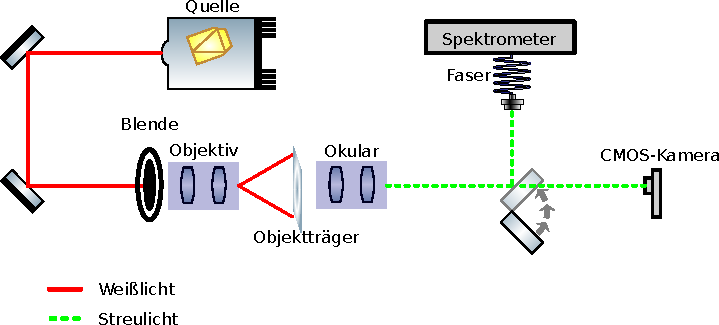
\includegraphics[width=\textwidth]{plots/dfm.PDF}
  \caption{Schemazeichnung des verwendeten Dunkelfeldmikroskop.}
  \label{fig:aufbau}
\end{figure}
Im Versuch wird als Beleuchtung eine Weißlichtquelle verwendet, welche über Silberspiegel in den Aufbau eingekoppelt wird. Anschließend wird der Lichtstrahl durch Lochblenden und Kollimatoren passend auf die Zentralblende (Durchmesser: $\SI{20}{\milli\meter}$, Ringbreite: $\SI{300}{\micro\meter}$) geführt. Als Objektiv wird ein Mikroskopobjektiv mit einer Numerischen Apertur von $0.9$ und 60-facher Vergrößerung bei einem Arbeitsabstand von $\SI{0.2}{\milli\meter}$ gewählt. Für das Okular wird ein weiteres Mikroskopobjektiv mit 50-facher Vergrößerung und Numerischer Apertur $0.5$ sowie einem Arbeitsabstand von $\SI{10.6}{\milli\meter}$ verwendet. Das entstehende Bild wird mit einer CMOS-Kamera in Echtfarbe aufgenommen und auf einem PC dargestellt. Um Spektren des gestreuten Lichts aufzunehmen kann hinter dem Okular ein Klappspiegel eingesetzt werden, mit dessen Hilfe das Licht in eine Glasfaser und so in ein Spektrometer geführt wird. Für Messungen der Polarisationsabhängigkeit des Streulichtes, wird vor der Zentralblende ein Polarisator in Form eines Glan-Taylor Prismas eingesetzt, mit dem die Polarisation des eingestrahlten Weißlichts gedreht werden kann.\\
\\
Mithilfe des Dunkelfeldmikroskops werden Bilder und Spektren von einer Probe mit Gold-Nanoröhrchen mit $25\times60 \si{\nano\meter}$ Dimension, sowie von Gold-Nanosphären aufgenommen. Die Nanopartikel sind auf einem gläsernen Objektträger aufgebracht. Es werden für beide Proben Bilder mit unterschiedlich hohen Teilchenzahlen aufgenommen. Außerdem werden für die Nanoröhrchen Spektren bei unterschiedlich polarisiertem Eingangslicht aufgenommen. \cite{anleitung}
%
% einfang only streulicht
% kein licht der quelle
% Aufbau
% hohe numerische apertur für eingang, damit weit aufgeweitet
% blende
% hinten etwas weniger, damit nur streu rein
% fotos?
% weisslicht
% cmos kamera
% spektrometer
%
% spektren von röhren und partikeln
% bilder
% bilder polabh.
% bilder intensitätsabh
